\documentclass[12pt]{article}
\usepackage[top=2.5cm, bottom=2.5cm, left=3cm, right=3cm]{geometry}
\usepackage{graphicx}
\begin{document}

\begin{Huge}
\begin{center}
\begin{normalsize}
\textbf{MAKERERE 
\includegraphics[scale=0.5]{logo} UNIVERSITY }\\


\textbf{FACULTY OF COMPUTING AND INFORMATICS TECHNOLOGY} \\
\textbf{SCHOOL OF COMPUTING AND INFORMATICS TECHNOLOGY} \\
\textbf{DEPARTMENT OF COMPUTER SCIENCE} \\
\textbf{BACHELOR OF SCIENCE IN COMPUTER SCIENCE} \\
\textbf{YEAR 2} \\
\textbf{BIT 2207 RESEARCH METHODOLOGY} \\
\textbf{Course Work: Assignment 3}\\
\end{normalsize}
\end{center}
\end{Huge}

\begin{center}
\begin{tabular}{|l|l|l|c|}
\hline NAME  & REG NO & STD NO \\\hline
OKOT EMMANUEL& 16/U/10916/PS & 216015844 \\\hline
\end{tabular}

\end{center}

\newpage

\begin{center}
\textbf{ROAD TRAFFIC ACCIDENTS IN UGANDA}\\
\paragraph{•}
Prepared by: OKOT EMMANUEL\\
\paragraph{•}
Lecturer: ERNEST MWEBAZE \\
\paragraph{•}
7th January 2018

\end{center}

\section{Abstract}
\paragraph{•}
There is a growing concern about the rising trend in mortality and morbidity from road traffic accidents in developing countries due to their effect on health care resources and budgets. Traffic accident injuries account for high medical care costs and loss of productivity.

\section{Introduction}
\paragraph{•}
Road traffic accidents are one of the leading causes of injuries and death in both developed and developing countries, and for both women and men. Traffic accidents are predictated to become the second leading cause of death in developing countries by the year 2020 (New Scientist, 1996); a remarkable rise from the eleventh leading cause of death in 1990. 
\paragraph{•}
Modernization has been accompanied by an increase in the number of vehicles on the road and vehicle ownership. The relationship between vehicle ownership and accident fatalities has been of interest to researchers.
\paragraph{•}
The document below describes the kind of data to be collected during research about road accidents. It also includes sample data that was collected during research.

\section{Data Form}
\paragraph{•}
In this research, data and information was collected by observation from scenes and interviews from people present at the accident scenes. The following describe the data that was collected from the forms:
\subsection{Location of Accident}
\paragraph{•}
This field enables one to input the name of the place where an accident has occurred.
\subsection{Image of Accident}
\paragraph{•}
This field is to enable one to upload an image of the scene.
\subsection{GPS Coordinates of the Place where the Accident Has Occurred}
\paragraph{•}
This field is to input the geographical location where the accident occurred.
\subsection{Enter Time and Date the Accident Has Occurred}
\paragraph{•}
This field is to input the date when the accident occurred.
\subsection{Car Model 1}
\paragraph{•}
This field is to enter the model of the car that caused the accident.
\subsection{Car Model 2}
\paragraph{•}
This field is to enter the model of the car that fell a victim of the accident.
\subsection{Sex of Driver that Caused the Accident}
\paragraph{•}
This field is to enter the sex of the driver that caused the accident.
\subsection{Age of the Driver that Caused the Accident}
\paragraph{•}
This field is to enter the age of the driver that caused the accident.
\subsection{Number of Passengers}
\paragraph{•}
This field is to enter the total number of passengers that were involved the accident.
\subsection{Number of Casualties}
\paragraph{•}
This field is to enter the number of casualties in an accident.
\subsection{Number of On-Spot Death Victims}
\paragraph{•}
This field is to enter the number of victims that have been involved in the accident and died on the scene.

\section{Sample Form}
\paragraph{•}
\textbf{Location of Accident}\\
Masaka

\paragraph{•}
\textbf{Image of Accident}\\
\begin{figure}
		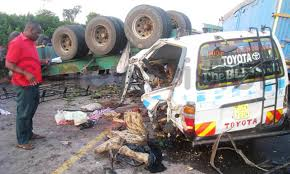
\includegraphics[scale=0.9]{images.jpg} 
			\end{figure}

\paragraph{•}
\textbf{GPS Coordinates of the place where the accident has occurred}\\
GPS Latitude: -0.3352 \\
GPS Longitude: 31.7341\\
GPS Altitude: 1278\\
GPS Accuracy: 19\\

\paragraph{•}
\textbf{Enter time and date the accident has occurred}\\
Sat Jun 24 00:00:00 UTC 2017


\paragraph{•}
\textbf{Car Model 1}\\
Commuter Taxi

\paragraph{•}
\textbf{Car Model 2}\\
Toyota Premio

\paragraph{•}
\textbf{Sex of Driver that Caused the Accident}\\
Male

\paragraph{•}
\textbf{Age of the Driver that Caused the Accident}\\
33

\paragraph{•}
\textbf{Number of passengers}\\
20

\paragraph{•}
\textbf{Number of casualties}\\
11

\paragraph{•}
\textbf{Number of on-spot death victims}\\
9

\end{document}